\documentclass{ctexart}
\usepackage{etex}
\usepackage{tikz}
\usetikzlibrary{arrows.meta}
\usetikzlibrary{calc} % 声明使用 calc 库

\begin{document}


We are working on
\begin{tikzpicture}
\draw (-1.5,0) -- (1.5,0);
\draw (0,-1.5) -- (0,1.5);
\end{tikzpicture}.



    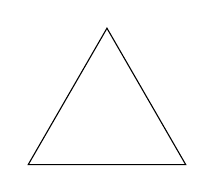
\begin{tikzpicture}
    % 定义正三角形的三个顶点
    \coordinate (A) at (0,0);
    \coordinate (B) at (2,0);
    \coordinate (C) at (1,{sqrt(3)});
    % 绘制正三角形
    \draw (A) -- (B) -- (C) -- cycle;
    \end{tikzpicture}




    \section{解三角形}
    \begin{tikzpicture}
        % 定义三角形的顶点
        \coordinate (A) at (0,0);
        \coordinate (B) at (7,0);
        % 使用余弦定理计算顶点 C 的位置
        \pgfmathsetmacro{\angleA}{acos((3*3 + 7*7 - 5*5)/(2*3*7))} %计算角度

        \coordinate (C) at ($(A)+({\angleA}:3)$);
        % 这是一个使用 calc 库的坐标计算表达式,具体解释如下:
        % $(A)$:表示已经定义好的坐标点 A 的位置。
        % +:代表向量加法运算。这里意味着要从点 A 出发,沿着某个方向进行移动。
        % ({\angleA}:3):这是一个极坐标表示法。在极坐标中,一个点的位置由角度和距离来确定。其中,\angleA 是之前通过 \pgfmathsetmacro 命令计算得到的角度(以弧度为单位),它表示从水平轴正方向开始逆时针旋转的角度;3 表示从点 A 出发沿着该角度方向移动的距离。

        % 绘制三角形
        \draw (A) -- (B) -- (C) -- cycle;
        
        % 标记顶点
        \node[below left] at (A) {$A$};
        \node[below right] at (B) {$B$};
        \node[above] at (C) {$C$};
        
        % 标记边长
        \node[below] at ($(A)!0.5!(B)$) {$7$};
        \node[ above right] at ($(B)!0.5!(C)$) {$5$};
        \node[ above left] at ($(A)!0.5!(C)$) {$3$};
    \end{tikzpicture}







    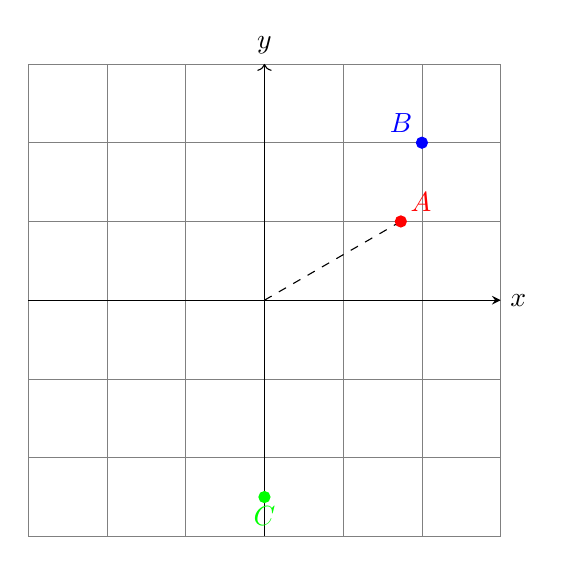
\begin{tikzpicture}
        % 设置网格,方便观察坐标位置
        \draw[help lines] (-3,-3) grid (3,3);
        % 绘制 x 轴和 y 轴
        \draw[-stealth] (-3,0) -- (3,0) node[right] {$x$};
        \draw[->] (0,-3) -- (0,3) node[above] {$y$};
    
        % 使用极坐标绘制点
        \coordinate (O) at (0,0);
        \coordinate (A) at (30:2); % 角度 30 度,距离原点 2 个单位
        \coordinate (B) at (45:{sqrt(8)}); % 角度 120 度,距离原点 1.5 个单位
        \coordinate (C) at (270:2.5); % 角度 270 度,距离原点 2.5 个单位
        \draw[dashed] (O) -- (A); %使用虚线
    
        % 绘制点并标记
        \filldraw[red] (A) circle (2pt) node[above right] {$A$};
        \filldraw[blue] (B) circle (2pt) node[above left] {$B$};
        \filldraw[green] (C) circle (2pt) node[below] {$C$};
    \end{tikzpicture}

    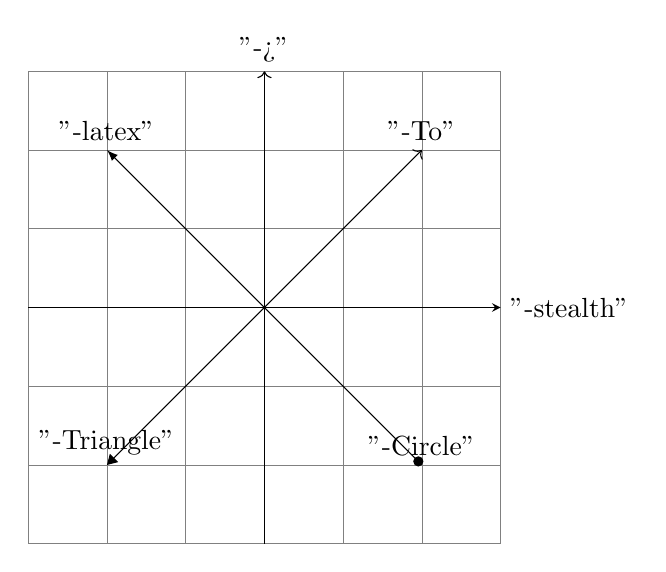
\begin{tikzpicture}
        % 设置网格,方便观察坐标位置
        \draw[help lines] (-3,-3) grid (3,3);
        % 绘制 x 轴和 y 轴
        \draw[-stealth] (-3,0) -- (3,0) node[right] {"-stealth"};
        \draw[->] (0,-3) -- (0,3) node[above] {"->"};
        \draw[-To] (0,0) -- (2,2) node[above] {"-To"};
        
        \draw[-latex] (0,0) -- (-2,2) node[above] {"-latex"};
        
        %\usetikzlibrary{arrows.meta}
        \draw[-Triangle] (0,0) -- (-2,-2) node[above] {"-Triangle"};
        \draw[-Circle] (0,0) -- (2,-2) node[above] {"-Circle"};
    \end{tikzpicture}

\section{圆}


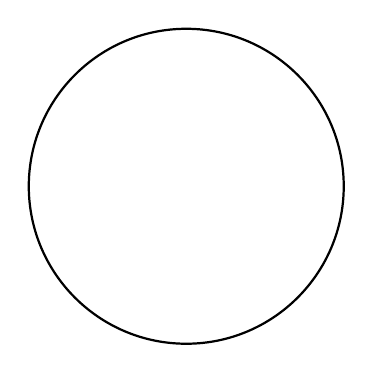
\begin{tikzpicture}
    % 绘制一个圆心在(0,0),半径为2cm的圆
    \draw[thick] (0,0) circle (2cm);
\end{tikzpicture}

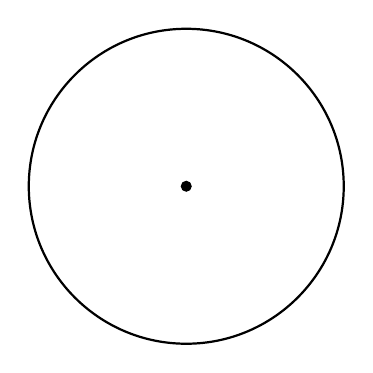
\begin{tikzpicture}
    \draw[thick] (0,0) circle (2cm);
    % 绘制一个圆心在(0,0),半径为2cm的圆
        % 绘制圆心的点
    \fill[black] (0,0) circle (2pt);
;

\end{tikzpicture}


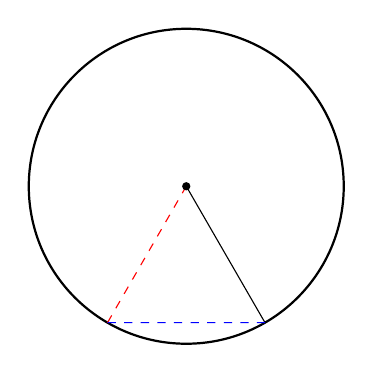
\begin{tikzpicture}
    % 绘制一个圆心在(0,0),半径为2cm的圆
    \coordinate (C) at (0,0); %这个点是圆心
    \draw[thick] (0,0) circle (2cm);
    \coordinate (A) at ($(C)+(-60:2)$); %使用带角度的极坐标
    \draw (A) -- (C);
    \coordinate (B) at ($(C)+(-{2*pi/3}r:2)$); %使用带弧度的极坐标,注意负号位置,({-pi/4}r:2)会报错
    \draw[dashed,red] (B) -- (C);
    \draw[dashed,blue] (B) -- (A);
    \fill[black] (C) circle (1.5pt); %绘值圆心的点
\end{tikzpicture}

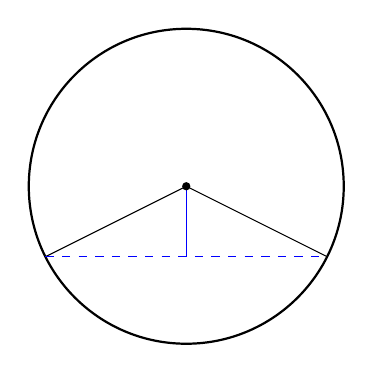
\begin{tikzpicture}
    % 绘制一个圆心在(0,0),半径为2cm的圆
    \coordinate (C) at (0,0); %这个点是圆心
    \draw[thick] (0,0) circle (2cm);
    \coordinate (A) at ($(C)+(-{atan(1/2)}:2)$); %使用带角度的极坐标
    \draw (A) -- (C);
    \coordinate (B) at ($(C)+({-180+atan(1/2)}:2)$);
    \draw (B) -- (C);
    \draw[dashed,blue] (B) -- (A);
    \coordinate (M) at ($(A)!0.5!(B)$);%计算中点
    \draw[blue] (M) -- (C);
    \fill[black] (C) circle (1.5pt); %绘值圆心的点
\end{tikzpicture}



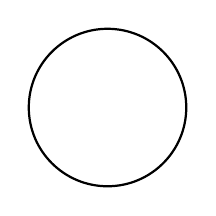
\begin{tikzpicture}

    % 绘制一个圆心在(0,0),半径为2cm的圆
    \draw[thick] (0,0) circle (1cm);
\end{tikzpicture}



\section{椭圆}
    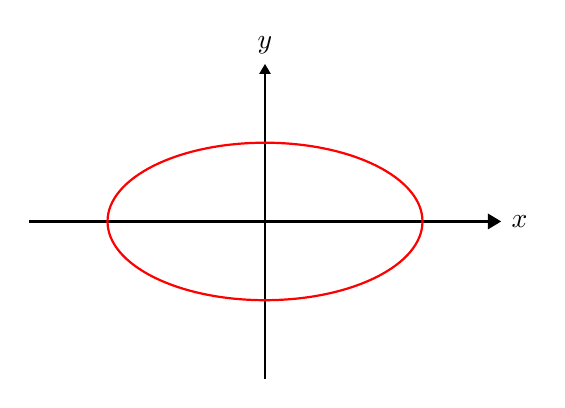
\begin{tikzpicture}[scale = 1]
        % 绘制坐标轴
        \draw[-Triangle,thick] (-3,0) -- (3,0) node[right] {$x$};
        \draw[-Triangle]  (0,-2) -- (0,2) node[above] {$y$};
    
        % 绘制椭圆
        \draw[ red, thick] (0,0) ellipse (2 and 1);
    
        % 标注椭圆的长半轴和短半轴
        % \draw[dashed] (0,0) -- (2,0) node[midway,below] {$a = 2$};
        % \draw[dashed] (0,0) -- (0,1) node[midway,left] {$b = 1$};
    \end{tikzpicture}

\section{双曲线}

$a = 1,b = 1$的时候,这里的双曲线是用参数方程定义的


\begin{figure}
    \centering
    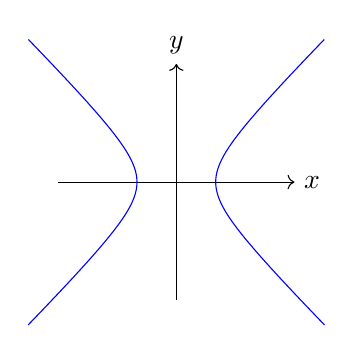
\begin{tikzpicture}[scale = 0.5]
        % 定义双曲线的参数
        \def\a{1}
        \def\b{1}
        % 绘制坐标轴
        \draw[->] (-3,0) -- (3,0) node[right] {$x$};
        \draw[->] (0,-3) -- (0,3) node[above] {$y$};
        % 绘制双曲线右支
        \draw[domain=-2:2, samples=100, smooth, variable=\t, blue] plot ({\a*cosh(\t)}, {\b*sinh(\t)});
        % 绘制双曲线左支
        \draw[domain=-2:2, samples=100, smooth, variable=\t, blue] plot ({-\a*cosh(\t)}, {\b*sinh(\t)});
    \end{tikzpicture}
    
\end{figure}

\begin{tikzpicture}[scale = 1]
    % 定义参数 p 的值
    \def\p{1/2}
    \def \x{1.2}
    % 绘制坐标轴
    \draw[->] (-0.2,0) -- (2,0) node[right] {$x$};
    \draw[->] (0,-1) -- (0,1) node[above] {$y$};
    % 绘制抛物线
    \draw[domain=-\x:\x, samples=100, smooth, variable=\t, blue] plot ({2*\p*\t*\t}, {2*\p*\t});
\end{tikzpicture}
\end{document} 